\documentclass[10pt]{article}

%\usepackage{hyperref}
\usepackage{alltt}
\usepackage{natbib}
\usepackage{graphicx}
\usepackage{url}
\usepackage{fancyhdr}
\usepackage{trust}
\pagestyle{fancy}

\lhead{}
\rhead{}
\lfoot{\copyright The University of Kansas, 2012}
\cfoot{\thepage}


\newtheorem{conjecture}{Conjecture}
\newtheorem{obligation}{Obligation}
\newtheorem{definition}{Definition}


\usepackage{ifthen}
\newboolean{submission}  %%set to true for the submission version
\setboolean{submission}{false}
%\setboolean{submission}{true}
\ifthenelse
{\boolean{submission}}
{ \newcommand{\todo}[1]{ } } % hide todo
{ \newcommand{\todo}[1]{ % show todo
   \marginpar{\raggedright\footnotesize{#1}}
               }}

\parskip=\medskipamount
\parindent=0pt

\bibliographystyle{abbrvnat}

\title{TPM Specification Design}
\author{Perry Alexander \and Brigid Halling}

\begin{document}

\maketitle
\tableofcontents
\listoffigures
\listoftables

\begin{abstract}
  The abstract goes here...
\end{abstract}

\section{Introduction}

\section{Modeling Approach}

\subsection{TPM Abstract State}

Figure~\ref{fig:tpm-abs-state} is the PVS record structure used to
represent the internal state of the TPM and necessary external state
of the environment it is running in.

\begin{figure}
\begin{alltt}
  tpmAbsState : TYPE = [#
                       memory : mem,
                       postInit : bool,
                       srk : (asymKey?),
                       ek : (asymKey?),
                       keys : KEYSET,
                       pcrs : PCRS,
                       locality : LOCALITY
                       #];
\end{alltt}
\caption{Abstract TPM and system state record data structure.}
\label{fig:tpm-abs-state}
\end{figure}

\subsection{TPM Abstract Command Definitions}

Figure~\ref{fig:tpm-command} is the PVS data type used to represent
the abstract syntax of the TPM command set.

\begin{figure}
\begin{footnotesize}
\begin{alltt}
  tpmInput : DATATYPE
  BEGIN
  %% Startup commands
    ABS_Init : ABS_Init? 
    ABS_Startup : ABS_Startup? % Only clear implemented
    ABS_SaveState : ABS_SaveState? % unimplemented
  %% PCRs, seals and keys
    ABS_Extend(h:HV,i:PCRINDEX) : ABS_Extend?
    ABS_Unseal(s:(sealBlob?),uk:(asymKey?)) : ABS_Unseal?   
    ABS_Seal(sk:(asymKey?),data:BLOB) : ABS_Seal?
    ABS_LoadKey2(lk:(wrapKey?)): ABS_LoadKey2? 
    ABS_CreateWrapKey(wk,parentk:(asymKey?)): ABS_CreateWrapKey?
  %% Quotes and Identities
    ABS_Quote(aik:(wrapKey?),nonce:BLOB,pm:PCRMASK) : ABS_Quote?
    ABS_MakeIdentity(naik:(asymKey?),k:(symKey?)) : ABS_MakeIdentity?
    ABS_ActivateIdentity(caik:(wrapKey?),k:(symKey?)) : ABS_ActivateIdentity?
  %% Ownership management
    ABS_TakeOwnership : ABS_TakeOwnership?
    ABS_OwnerClear : ABS_OwnerClear? % unimplemented
    ABS_ForceClear : ABS_ForceClear? % unimplemented
    ABS_DisableOwnerClear : ABS_DisabelOwnerClear? % unimplemented
  %% Software Commands
    ABS_senter : ABS_senter? % implemented all actions as one senter
    ABS_sinit : ABS_sinit? % partially implemented
    ABS_Save(i:nat,v:tpmAbsOutput) : ABS_Save?
    ABS_Read(i:nat) : ABS_Read?
  %% CA Commands
    ABS_certify(aik:(wrapKey?),ek:(asymKey?),freshk:(symKey?)) : ABS_certify?
  %% Invented, imaginary Commands
    noopCom : noopCom?
  END tpmInput;
\end{alltt}
\end{footnotesize}
\caption{TPM command data type.}
\label{fig:tpm-command}
\end{figure}

Table~\ref{tab:tpm-to-pvs} maps TPM concrete commands to their
abstract PVS representations.

\begin{table}[hbtp]
  \centering
  \begin{tabular}{lll}
    \hline
    \emph{TPM} & \emph{Abstract PVS} & \emph{Concrete PVS} \\
    \emph{Command} & \emph{Command} & \emph{Command} \\ \hline
    \multicolumn{3}{l}{\emph{Startup}}  \\ \hline
    \textsf{TPM\_Init} & \verb+ABS_Init+ & \\ 
    \textsf{TPM\_Startup} & \verb+ABS_Startup+ & \\
    \textsf{TPM\_SaveState} & \verb+ABS_SaveState+ & \\ \hline
    \multicolumn{3}{l}{\emph{PCRs, seals and keys}}  \\ \hline
    \textsf{TPM\_Extend} & \verb+ABS_Extend(h,i)+ & \\
    \textsf{TPM\_Seal} & \verb+ABS_Seal(sk,data)+& \\
    \textsf{TPM\_Bind} & & \\
    \textsf{TPM\_Unbind} & & \\
    \textsf{TPM\_Unseal} & \verb+ABS_Unseal(s,uk)+ & \\
    \textsf{TPM\_CreateWrapKey} & \verb+ABS_CreateWrapKey(wk,parentk)+ & \\
    \textsf{TPM\_LoadKey2} & \verb+ABS_LoadKey2(k)+ & \\ \hline
    \multicolumn{3}{l}{\emph{Quotes and Identities}}  \\ \hline
    \textsf{TPM\_Quote} & \verb+ABS_Quote(aik,b,pm)+ & \\
    \textsf{TPM\_MakeIdentity} & \verb+ABS_MakeIdentity(naik,k)+ & \\
    \textsf{TPM\_ActivateIdentity} & \verb+ABS_ActivateIdentity(caik,k)+ & \\
    \multicolumn{3}{l}{\emph{Ownership}}  \\ \hline
    \textsf{TPM\_TakeOwnership} & \verb+ABS_TakeOwnership+ & \\ \hline
    \textsf{TPM\_OwnerClear} & & \\
    \textsf{TPM\_ForceClear} & & \\ 
    \textsf{TPM\_DisableOwnerClear} & & \\
    \hline
  \end{tabular}
  \caption{TPM command mapping to PVS command representation.}
  \label{tab:tpm-to-pvs}
\end{table}

Table~\ref{tab:commands-to-pvs} maps external commands that interact
with the TPM to their PVS representations.

\begin{table}[hbtp]
  \centering
  \begin{tabular}{lll}
    \hline
    \emph{External}& \emph{Abstract PVS} & \emph{Concrete PVS} \\
    \emph{Command} & \emph{Command} & \emph{Command} \\ \hline
    \textsf{senter} & \verb+ABS_senterCom+ & \\
    \textsf{sinit} & \verb+ABS_sinitCom+ & \\
    Save to memory & \verb+ABS_Save(i,v)+ & \\
    Read from memory & \verb+ABS_Read(i)+ & \\
    CA certification & \verb+ABS_certify(aik,ek,freshk)+ & \\
    Power On & \verb+powerCom+ & \\
    Power Off  & \verb+offCom+ & \\
    \hline
  \end{tabular}
  \caption{System commands interacting with TPM.}
  \label{tab:commands-to-pvs}
\end{table}

\subsection{TPM Abstract Outputs}

\begin{figure}[hbtp]
  \begin{footnotesize}
  \begin{alltt}
  tpmAbsOutput : DATATYPE
  BEGIN
    outNothing : outNothing?
    outError(errorVal:nat) : outError?
    outQuote(oqk:KEY,oqnon:BLOB,oqpcrs:list[PCR]) : outQuote?
    outWrapKey(owk:KEY) : outWrapKey?
    outAsymKey(oask:KEY) : outAsymKey?
    outSymKey(osk:KEY) : outSymKey?
    outBlob(obl:BLOB) : outBlob?
    outCertReq(ocertaik:(wrapKey?),ocertek:(asymKey?),ofreshk:(symKey?)) : outCertReq?
    outIdentity(oidentaik:(wrapKey?),oidentc:(outCertReq?)) : outIdentity?
    outIdentActivation(oactc:(certBlob?),osessk:(symKey?),oactek:(asymKey?)) : outIdentActivation?
    outFullQuote(ofullqc:(certBlob?),ofullqsml:SML,ofullqq:(outQuote?)) : outFullQuote?
    outPCR(pcr:PCR) : outPCR?
  END tpmAbsOutput;
  \end{alltt}
  \end{footnotesize}
  \caption{Abstract TPM outputs}
  \label{fig:tpm-abs-output}
\end{figure}

\subsection{Defining Abstract TPM Command Execution}

The technique for specifying TPM command execution is to define a
transition from \verb+tmpAbsState+ (figure~\ref{fig:tpm-abs-state})
and \verb+tpmInput+ (figure~\ref{fig:tpm-command}) to
\verb+tpmAbsState+:

\begin{alltt}
  executeCom : tpmAbsState \(\rightarrow\) tpmInput \(\rightarrow\) tpmAbsState
\end{alltt}

\noindent and a transition from \verb+tmpAbsState+
(figure~\ref{fig:tpm-abs-state}) and \verb+tpmInput+
(figure~\ref{fig:tpm-command}) to \verb+tpmAbsOutput+:

\begin{alltt}
  outputCom : tpmAbsState \(\rightarrow\) tpmInput \(\rightarrow\) tpmAbsOutput
\end{alltt}

Given $s:tpmAbsState$ and $c:tpmAbsInput$ the output, state pair
resulting from executing $c$ are defined as:

\begin{alltt}
  (outputCom(\(s\),\(c\)),executeCom(\(s\),\(c\)))
\end{alltt}

This is a standard technique for defining state transition and output
functions for any transition system.

As one would expect, \verb!executeCom! and \verb!outputCom! are
defined by cases over \verb!tpmAbsInput!.  For each command in
\verb!tpmAbsInput! a function is defined for generating the next state
and for generating output.  These commands are named within the
specification using the suffix \verb!State! and \verb!Out!
respectively for easy identification.

As a concrete example, consider the \verb!ABS_ActivateIdentity!
input.  The function \verb!activateIdentityState! defines how the TPM
state is modified:

\begin{alltt}
    activateIdentityState(s:tpmAbsState,a:(wrapKey?),k:(symKey?)) : tpmAbsState =
    loadKey2State(s,a);
\end{alltt}

\noindent while, the function \verb!activateIdentityOut! defines
the TPM output generated by the command:

\begin{alltt}
  activateIdentityOut(s:tpmAbsState,a:(wrapKey?),k:(symKey?)) : tpmAbsOutput =
    IF checkKeyRoot(a,srk(s)) THEN outSymKey(k) ELSE outNothing ENDIF;
\end{alltt}

Note that many commands in the current abstract model either modify
state or generate output.  In such cases only the pertinent function
is defined with the \verb!CASES! construct used to assemble the
functions defaulting to not modifying the state and generating a null
output.

\subsection{Sequencing TPM Commands}

Sequencing of TPM commands is a matter of using the output state from
one command as the input to the next command.  The classical mechanism
for doing this involves executing a command and manually feeding its
outputs to the next state.  Using a \verb!LET! form, to execute
\verb!i;i'! would look like the following:\footnote{We use the
  semicolon in the canonical style to represent sequential execution.}

\begin{alltt}
  LET (s',o') = (executeCom(s,i),outputCom(s,i)) IN
    (executeCom(s',i'),outputCom(s',i'))
\end{alltt}

\noindent where the tick denotes next.

The notation typically used does not use the \verb!LET!, performing
calls directly:

\begin{alltt}
    (executeCom(executeCom(s,i),outputCom(s,i)),
     outputCom(executeCom(s,i),outputCom(s,i)))
\end{alltt}

TPM command execution is inherently sequential, making this notation
exceptionally obtuse and difficult manage.  Thus, we choose to use an
alternative approach that uses a \emph{state monad} to model
sequential execution.  In effect, the state monad threads the state
through sequential execution in the background.

To understand the state monad, lets first define a simple data type,
\verb!State!, having a single field called \verb!state! that holds a
function from an abstract state to an abstract state, abstract output
pair:

\begin{alltt}
 State : DATATYPE
 BEGIN
   state(runState:[tpmAbsState->[tpmAbsOutput,tpmAbsState]]):state?
 END State
\end{alltt}

Given $s$, a value of type \verb!tpmAbsState!, and $m$, a \verb!State!, the
application:

\begin{alltt}
  runState(m)(s)
\end{alltt}

\noindent will result in a \verb!tpmAbsOutput!, \verb!tpmAbsState!
pair.  This is precisely the output expected.  Note that the use of
\verb!State! and \verb!state! in this definition is somewhat
misleading.  Neither is actually a state, but a state monad that given
a state will generate a new state.  The data type should be viewed as
a kind of state generation or next-state function, not a single
state.\footnote{The notation used here is consistent with the
  literature.}

Two functions must be defined for any instance of a monad -- unit and
bind (\verb!>>=!).  We will also define sequence (\verb!>>!) command
that is a special case of bind commonly defined in most state monad
implementation.

First we define \verb!unit!, frequently called \verb!return! in the
literature.  It's form is:

\begin{alltt}
  unit(x:tpmAbsOutput):State = state(LAMBDA (s:tpmAbsState) : (x,s));
\end{alltt}

What \verb!unit! does is lift a member of \verb!tmpAbsState! into
\verb!State! -- given a \verb!tpmAbsState! it produces a \verb!State!.
Specifically, when \verb!unit! is provided with a \verb!tpmAbsState!
it should give back a \verb!State! whose \verb!runState! field should
simply produce it.

\verb!runState! is a function from \verb!tpmAbsState! to a
\verb!tpmAbsOutput!, \verb!tpmAbsState! pair.  Clearly, the state part
of the output should be the state lifted by \verb!unit!.  But what
about the output?  If we are lifting \verb!tpmAbsState! there is no
way to extract an output.  The \verb!bind! function handles this by
simply requiring an output be specified as a parameter.

Given an output value \verb!a!, \verb!unit(s)! evaluates asL

\begin{alltt}
  unit(a) = state(LAMBDA (s:tpmAbsState) : (a,s))
\end{alltt}

Recognize that the resulting value is of type \verb!State!.  This is
not a state, but a state monad that can produce a state.
Specifically, if we extract the \verb!runState! function and apply it
to a \verb!tpmAbsState! we will get the output, state pair that we
need.  Specifically:

\begin{alltt}
  runState(unit(a))(st) = runState(state(LAMBDA (s:tpmAbsState)) :  (a,s))(st);
                        = (LAMBDA (s:tpmAbsState) : (a,s))(st)
                        = (a,st)
\end{alltt}

The output specified when the monad was created, \verb!a!, is the
output included in the application.  No matter what \verb!tpmAbsState!
this \verb!runState! is applied to the output will always be
\verb!a!.  However, the state element of the output will always be the
state input to \verb!runState!.  So, we have a function that will
always produce a pair whose output value is \verb!a! and whose state
value is the state passed to it.  This is what we mean by lifting a
value into the state monad.

% \begin{alltt}
%   unit(\(a\)) = state(LAMBDA (\(s\):tpmAbsState) : (\(a\),\(s\)));
% \end{alltt}

Before moving on to bind and sequence, a quick note about how
\verb!unit! works may simplify things.  Applying \verb!unit! to a
\verb!tpmAbsState! value produces a state monad value.  In that value,
the output is hard wired by the application of \verb!unit! -- it is
provided as an input and the resulting monad carries it along.  This
is precisely how the monad will handle state.  With a bit more
machinery, we will use the state generated as a value in the monad
representing the next state.

The second function defined for all monads is bind, typically
represented by the infix operator \verb!>>=!.  The bind operation
takes a monad and a function from \verb!tpmAbsOutput! to a monad and
produces a new monad.  The signature is of the form:

\begin{alltt}
  m:State >>= f:[A->State] : State
\end{alltt}

Unfortunately, the signature alone provides little as to the actual
function of bind.  The implementation is:

\begin{alltt}
 >>= (m:State,f:[A->State]):State =
   state(LAMBDA(s0:S):
          LET (a,s1) = runState(m)(s0) IN 
	    runState(f(a))(s1));
\end{alltt}

Keep in mind that bind does not produce a state.  Instead it produces
a state monad that given a state will produce and output state pair.
That state is the parameter \verb!s0! in the above implementation.
The biggest clue to the behavior of bind comes in the \verb!LET! form
where \verb!(a,s1)! is bound to running \verb!m! -- the first argument
to bind -- on state \verb!s0!.  \verb!a! is bound to the output and
\verb!s1! to the state resulting from running \verb!m! on \verb!s0!.


\begin{alltt}
 >> (m:State,f:State):State =
   state(LAMBDA(s0:S):
          LET (a,s1) = runState(m)(s0) IN
            runState(f)(s1));
\end{alltt}

\section{Verification Approach}

The approach taken for verification is establishing a \emph{weak
  bisimulation}~\citep{Sangiorgi:12:Introduction-to} relation between
an abstract requirements model and a model derived from the TPM
specification as shown in figure~\ref{fig:bisimulation}.

\begin{figure}[hbtp]
  \centering
  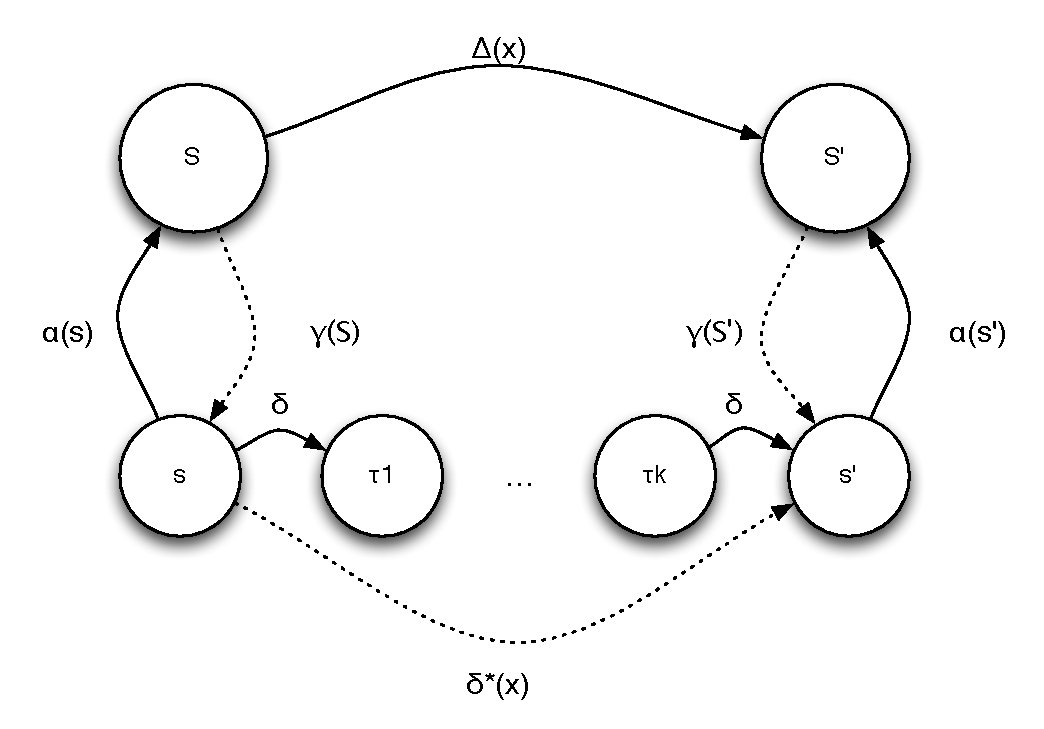
\includegraphics[width=0.75\textwidth]{figures/bisimulation.pdf}
  \caption{Weak bisimulation relation between an abstract transition
    system $A=(S,\Sigma,\Delta)$ and a concrete transition system
    $C=(s,\sigma,\delta)$.}
  \label{fig:bisimulation} 
\end{figure}

We say that $A=(S,\Sigma,\Delta)$ is an \emph{abstract model} where
$S$ is a set of abstract states, $\Sigma$ is a set of actions on
states and input, and $\Delta : S\times\Sigma\rightarrow\Sigma$ is a
transitions on state and action.  Similarly, we say that
$C=(s,\sigma,\delta)$ is a \emph{concrete state } where $s$ is a set
of concrete states, $\sigma$ is a set of actions on states and input,
and $\delta : s\times\sigma\rightarrow\sigma$ is a transition
function.

We relate the abstract and concrete models through an \emph{abstraction
function}, $\alpha:s\rightarrow S$, and \emph{concretization
function}, $\gamma:S\rightarrow 2^s$.  The abstraction and
concretization functions must form a Galois Connection such that:

\[s\in\gamma(\alpha(s))\]

\noindent Specifically, when making the result of an abstraction
concrete, the original state must be in the resulting set.  Note that
the concretization function may result in multiple states due to the
necessity of specifying unknown detail.

We say that $A$ and $C$ are weakly bisimilar ($A\sim C$) if when
$\alpha(s)=S$ then $\alpha(\delta^*(s))=\Delta(S)$ for all inputs to
$s$.

\begin{definition} 
  \[A\sim C \equiv \forall s_0:s \cdot \exists S_0:S \cdot
  \alpha(s_0)=S_0 \Rightarrow \alpha(\delta^*(s_0))=\Delta(S_0)\]
  \label{def:bisimulation}
\end{definition}

In the formal TPM model \texttt{tpmAbsState} defines $S$ while
\texttt{tpmConcState} defines $s$.

\appendix

\chapter{Glossary}
\label{chapt:glossary}

This glossary is intended to document some common acronyms as well as
define some common terms.  It is currently a bit haphazard and a
number of elements are missing.

\section{Trusted Platform Definitions}

\begin{description}
  \parskip=0pt
  \itemsep=\smallskipamount
\item[Trusted Platform Module (TPM)] -- Hardware Trusted Platform
  Module as defined by TCG.
\item[Process Configuration Register (PCR)] -- Registers defined in
  the TPM.  In the TPM there are at least 16 and they are 20 bytes
  wide.
\item[Bound to PCR] -- Encryption including PCR values that must match
  TPM PCR values before decryption is performed.
\item[Sealed to State] -- Operation performed by the TPM where data is
  encrypted and bound to PCRs or a PCR composite that must be checked
  before unsealing.  Only data is sealed.
\item[Wrapped Key] -- An asymmetric key with its private key encrypted
  and its public key visible.  Only keys are wrapped.
\item[Virtual TPM (vTPM)] -- A virtual Trusted Platform Module
\item[Certified Key (CK)] - Asymmetric key with private key signed by the
  AIK private key.
\item[Endorsement Key (EK)] - Asymmetric key who's private key is in
  the TPM hardware.  Private key is used to sign data from TPM while
  public key is used to encrypt sensitive data sent to the TPM.  The
  EK is set by the TPM factory and may not be reset.
\item[Attestation Identity Key (AIK)] - Asymmetric key whose private
  key is used for only two purposes: (i) sign (or attest to) TPM
  internal state; (ii) sign (or certify) other general purpose keys.
  AIKs are generated by a TPM, certified by a trusted third party,
  and used for signing in lieu of the EK.
\item[Storage Root Key (SRK)] - Root of secure storage hierarchy.
  Used to encrypt storage keys that exist outside the TPM.  The SRK
  may be reset.
\item[Attestation Identity Certificate (AIC)] - Certificate
  provided by a trusted third party binding an AIK to a specific
  trusted platform.
\item[Digest] - 20-byte Value contained in a PCR.
\item[PCR Composite] - Single digest value generated from a collection
  of PCR values.
\item[Quote] - A value along with a set of PCR values or PCR composite
  signed by a TPM using an AIK.
\item[Root of Trust for Measurement (RTM)] - the ``place to stand''
  for measurement.  Effectively a hardware-based trusted launch point
  that will faithfully measure, start and pass control to its target
  without trusting other components.
\item[Root of Trust for Storage (RTS)] - the ``place to stand'' for
  measurement storage.  Effectively a trusted hardware store that will
  store measurements with integrity without trusting other components.
\item[Root of Trust for Reporting (RTR)] - the ``place to stand'' for
  generating quotes and providing evidence with integrity and
  authenticity.  Effectively a trusted hardware component that
  generates and signs quotes.
\end{description}

\section{Cryptography Notations}

\begin{description}
  \itemsep=0pt
  \parskip=\smallskipamount
\item[Hash Notation] $\hash{data}$ - The hash of $data$.
\item[Certificate Notation] $\cert{cert}{key}$ - Certificate, $cert$, signed by
  $key$.
\item[Signed Data Notation] $\sign{data}{key}$ - $data$, signed by $key$.
\item[Encrypted Data Notation] $\encrypt{data}{key}$ - $data$
  encrypted with $key$.
\item[Sealed Data Notation] $\seal{data}{pcrs}$ - $data$ sealed to
  $pcrs$.
\item[Wrapped Key Notation] $\wrap{k}{pcrs}$ - Equivalent to the key
  pair $(\seal{\private{k}}{pcrs},\public{k})$
\end{description}

\section{Intel Secure Boot}

\begin{description}
  \itemsep=0pt
  \parskip=\smallskipamount
\item[Trusted eXecution Technology (TXT)] - Intel's trusted boot
  support.
\item[Measured Launch Environment (MLE)] - Run time environment
  providing a measured boot.  Initialized and started by the SINIT
  command execution.
\item[SENTER or GETSEC] - Intel's trusted boot command.  Provides
  synchronization, special bus cycles, and a special environment
  residing on the CPU (ACEA).
\item[Secure INITialization Instructions (SINIT)] - Code for
  performing secure initialization.  Loaded by SENTER and validated by
  the ACM.
\item[Authenticated Code Execution Area (ACEA)] - CPU resident
  environment for executing code known as the Authenticated Code
  Module (ACM).  Boot sequence involving SENTER and SINIT is as
  follows:

  \begin{enumerate}
    \parskip=0pt\itemsep=0pt
  \item Load SINIT and MLE into memory
  \item Invoke SENTER (GETSEC)
  \item Establish special environment (ACEA)
  \item Load SINIT into ACEA
  \item Validate SINIT digital signature and store SINIT identity in
    TPM
  \item SINIT measures MLE in memory and stores MLE identity in TPM
  \item SINIT passes control to MLE
  \end{enumerate}

\item[Authenticated Code Module (ACM)] - Code running in the ACEA. May
  be used for validating platform configuration, measuring the
  measured launch environment, cleaning up after crashes.
\end{description}



%%\nocite{}

\bibliography{tpm-spec-design}

\end{document}
